% Preamble
\documentclass[11pt]{article}
% Packages
\usepackage{ngerman}
\usepackage{amsmath}
\usepackage{url}
\usepackage{graphicx}
\usepackage{float}
\usepackage{pifont}
% Title ToC

\title{\textbf{Konzepte} zur Bachelorarbeit\\\large{Template-basierte Synthese von\\Verzweigungsstrukturen mittels
L-Systemen}}
\author{Adrian Helberg}

% Document
\begin{document}
    \maketitle
    \tableofcontents
    \newpage
    \section{Literaturübersicht}
    \subsection{Softwaretechnik}
    Eine Fallstudie der Universität Karlsruhe~\cite{1} untersucht den Einsatz der Softwaretechnik \textbf{Extreme
    Programming}
    (XP) im Kontext der Erstellung von Abschlussarbeiten im Universitätsumfeld.
    Hierzu werden folgende Schlüsselpraktiken untersucht:
    \begin{itemize}
        \item XP als Softwaretechnik zur schrittweisen Annäherung an die Anforderungen eines Systems
        \item Änderung der Anforderungen an das Systems
        \item Funktionalitäten (\textbf{Features}) werden als Tätigkeiten des Benutzers (\textbf{User Stories}) definiert
        \item Zuerst werden Komponententests (Modultests) geschrieben und anschließend die Features (Test-driven Design)
        \item Keine seperaten Testing-Phasen
        \item Keine formalen Reviews oder Inspektionen
        \item Regelmäßige Integration von Änderungen
        \item Gemeinsame Implementierung (Pair Programming) in Zweiergruppen
    \end{itemize}
    Aus der Fallstudie geht hervor, dass Extreme Programming einige Vorteile bei der Bearbeitung eines Softwareprojektes
    einer Bachelorarbeit bietet.
    Zum einen können sich Anforderungen an das zu erstellende System durch parallele Literaturrecherche ändern, zum
    anderen können Arbeitspakete durch Releases abgebildet werden.

    \subsection{Grundlagen}
    \begin{itemize}
        \item L-Systeme~\cite{3}
        \item Turtle-Algorithmus~\cite{4}
        \item Parametrisierte L-Syteme~\cite{5}
        \item String matching~\cite{6}
        \begin{itemize}
            \item Verschiedene Algorithmen~\cite{7},~\cite{8}
        \end{itemize}
    \end{itemize}

    \subsection{Basisquelle}
    Bei \textit{Inverse Procedural Modeling of Branching Structures by Inferring L-Systems}\cite{2} geht es um ein
    Modell zum Lernen von L-Systemen von Verzweigungsstrukturen mithilfe maschinellen Lernens (\textit{Deep
    Learning}) anhand beliebiger Grafiken.
    Hierzu werden atomare Strukturen mit einem neuronalen Netz erkannt, eine hierarchische Topologie (Baumstruktur)
    aufgebaut, aus der ein L-System inferiert und mit einem \textbf{Greedy} Algorithmus optimiert wird.
    Ausgabe des Systems ist ein generalisiertes L-System, aus dem ähnliche Strukturen, wie die der Inputgrafik,
    erstellt werden können.\\
    Aus dieser Quelle werden folgende Konzepte genutzt:
    \begin{itemize}
        \item Nutzer einer Baumstruktur zur Organisation von genutzten atomaren Verzweigungsstrukturen
        (\textbf{Templates}) mit Knoten für Templates und Kanten für geometrische Transformationen
        \item Untersuchen der Baumstruktur auf Wiederholungen
        \item Parametrisierte L-Systeme (L-System mit \textbf{Modulen}) zur Abbildung von Transformationsparametern
        \item Kostenfunktion zur Bewertung eines L-Systems
    \end{itemize}


    \section{Eigenleistung}
    Die Eigenleistung der Bachelorarbeit besteht aus:
    \begin{itemize}
        \item Algorithmus Baumstruktur $\rightarrow$ L-System
        \item Leere Symbole ($\varepsilon$) als Dummy-Knoten für Terminale
        \item Parameterverteilung als Histogramm
        \item Gewichtetes Randomisieren von Parametern
    \end{itemize}

    \newpage

    \section{Dokumentation}
    \subsection{Gliederung}
    Im Folgenden wird eine vorläufige Gliederung der schriftlichen Ausarbeitung gezeigt
    \begin{itemize}
        \item[1.] Abbildungs- und Tabellenverzeichnis
        \item[2.] Abkürzungsverzeichnis
        \item[3.] Einleitung
        \begin{itemize}
            \item[3.1.] Problemstellung
            \item[3.2.] Ziele
            \item[3.3.] Methodik
            \item[3.4.] Aufbau
        \end{itemize}
        \item[4.] Grundlagen
        \begin{itemize}
            \item[4.1.] Grundbegriffe
            \item[4.2.] Grundlegende Arbeiten
            \item[4.3.] Verwandte Arbeiten
        \end{itemize}
        \item[5.] Konzepte
        \begin{itemize}
            \item[5.1.] Probleme \& Lösungsansätze
            \item[5.2.] Architektur
            \item[5.3.] Algorithmen
        \end{itemize}
        \item[6.] Implementierung
        \item[7.] Evaluierung
        \begin{itemize}
            \item[7.1.] Testumgebung
            \item[7.2.] Beobachtungen \& Ergebnisse
            \item[7.3.] Diskussion und Bewertung
        \end{itemize}
        \item[8.] Ausblick
        \item[9.] Literaturverzeichnis
        \item[10.] Eidesstattliche Erklärung
    \end{itemize}

    \section{Softwareprojekt}

    \subsection{Vorgehen}
    Das Programm zu dieser Arbeit wird mit einem XP-basierten Ansatz erarbeitet.
    Hierbei beinhaltet ein \textbf{Release} Funktionen, die insgesamt für eine neue Version des Systems ausreichen;
    also ein vollständig funktionsfähiges Programm liefern.
    \textbf{User Stories} sind innerhalb der Iterationen umzusetzende Teilaufgaben und deren Aufwandseinschätzung gibt
    Auskunft über den Entwicklungsaufwand einer Umsetzung.\\~\\
    Umsetzung des Softwareprojektes in Iterationen mit folgenden Phasen:
    \begin{itemize}
        \item Planung:
        \begin{itemize}
            \item Release-Planung:\\"`\textit{Welche Features werden in diesem Release umgesetzt?}"',\\User Stories,
            Aufwandsschätzung, Anforderungsmanagement
            \item Iterationsplanung:\\Umwandlung der User Stories in kleine Arbeitsschritte,\\Festlegen der Dauer einer
            Implementierung
        \end{itemize}
        \item Entwurf: Architektur, Klassendiagramme, Schnittstellen
        \item Testing: (Automatisierte) Modul- und Regressionstests
        \item Programmierung: Umsetzung der Features, Implementierung, Modularisierung
    \end{itemize}
    \begin{figure}[H]
        \centering
        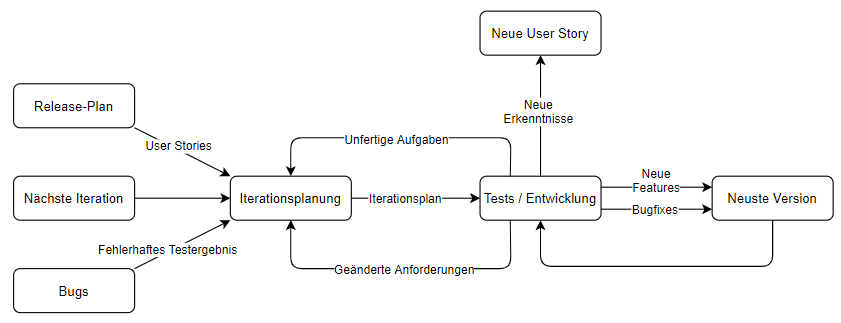
\includegraphics[width=15cm]{../images/extreme_programming.PNG}
        \caption{Ablaufdiagramm}
    \end{figure}

    \subsection{Technnologien}
    \begin{itemize}
        \item Programmiersprache: Java Version X mit
        \begin{itemize}
            \item JavaFX Version X
        \end{itemize}
        \item Build-Management-Tool: Gradle\cite{gradle} Version X
        \item Versionskontrolle: Github Repository\cite{github} via Git\cite{git}
        \item IDE: JetBrains IntelliJ IDEA\cite{idea} 2020.2.2 (Ultimate Edition)
        \item Betriebssystem: Microsoft Windows 10 Pro 64 Bit
        \item Prozessor: Intel Core i5-3570K CPU @ 3.40GHz
        \item User Story Map: Trello Board\cite{trello}
    \end{itemize}

    \newpage

    \section{Softwarearchitektur}
    Die Gliederung der Inhalte für die Softwarearchitektur erfolgt nach der arc42-Vorlage~\cite{arc42}

    \subsection{Einführung und Ziele}
    Ziel ist die Erstellung eines Programms zur Synthetisierung von Ähnlichkeitsabbildungen einer vom Benutzer
    erstellten Verzweigungsstruktur mittels Inferieren und Optimieren von L-Systemen.
    Die wesentlichen Features des Programms sind:
    \begin{itemize}
        \item Erstellung einer Verzweigungsstruktur über eine grafische Benutzeroberfläche (\textbf{GUI})
        \item Einbindung atomarer Strukturen über externe Dateien
        \item Synthetisierung von ähnlichen Verzweigungsstrukturen anhand der erstellten Struktur
        \item Anzeigen von Verzweigungsstrukturen
    \end{itemize}
    Priorisierte (absteigend) Qualitätsziele, die bei der Erstellung des Systems umgesetzt werden sollten:
    \begin{itemize}
        \item \textbf{Funktionalität} durch Umsetzung aller Teilsysteme
        \item \textbf{Interoperabilität} durch Nutzen einer allgemeinen Repräsentation von L-Systemen, damit diese
        auch in anderen Programmen oder Algorithmen verwendet werden kann
        \item \textbf{Erweiterbarkeit} durch offene Entwurfsmuster (Design Pattern)
        \item \textbf{Modular}e Implementierung für effiziente Wartung und Erweiterung
        \item \textbf{Effizienz} durch effiziente Programmierung
        \item \textbf{Attraktivität} durch intuitive Benutzung (Benutzerfreundlichkeit)
        \item \textbf{Plattformunabhängigkeit} durch Verwenden des Java-Frameworks
    \end{itemize}

    \subsection{Kontextabgrenzung}
    \begin{figure}[H]
        \centering
        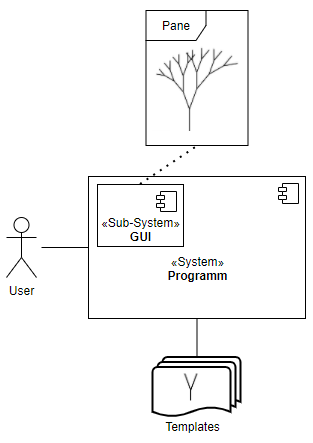
\includegraphics[width=6.2cm]{../images/Fachlicher_Kontext.PNG}
        \caption{System und Systemumgebung}
    \end{figure}
    \begin{figure}[H]
        \centering
        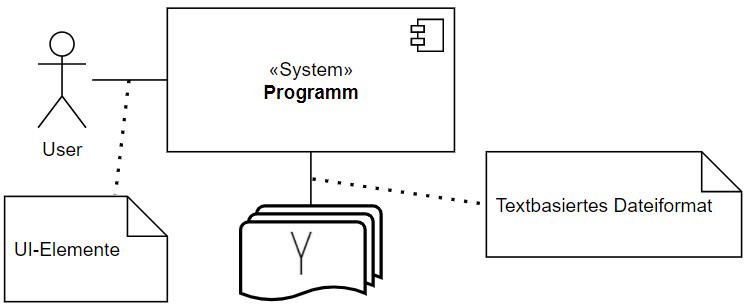
\includegraphics[width=10cm]{../images/Technischer_Kontext.PNG}
        \caption{Technische Interaktion zwischen System und Systemumgebung}
    \end{figure}

    \newpage

    \subsection{Lösungsstrategie}
    Gewählte Architekturansätze zur Erreichung der Qualitätsziele:
    \begin{center}
        \begin{tabular}{l|l}
            \textbf{Qualitätsziel} & \textbf{Architekturansatz} \\
            \hline \\
            Funktionalität &
            \begin{minipage}[t]{0.8\textwidth}
                \begin{itemize}
                    \item Grafische Benutzerschnittstelle: \textit{GUI}
                    \item Generieren der Baumstruktur: \textit{TreeGenerator}
                    \item Ableiten von L-Systemen aus Baumstrukturen: \textit{Inferer}
                    \item Generalisieren von L-Systemen: \textit{Generalizer}
                    \item Randomisieren von L-System Parametern: \textit{Randomizer}
                \end{itemize}
            \end{minipage} \\
            \\ \hline \\
            Interoperabilität &
            \begin{minipage}[t]{0.8\textwidth}
                Durch das Nutzen allgemeingültiger mathematischer Beschreibungen sollen erstellte
                L-Systeme in Fremdsystemen, wie Online Visualisierer, genutzt werden können
            \end{minipage} \\
            \\ \hline \\
            Erweiterbarkeit &
            \begin{minipage}[t]{0.8\textwidth}
                Das Nutzen des \textbf{Pipeline Design Pattern}s soll das Erweitern des Systems durch
                Hinzufügen weiterer Teilschritte (\textbf{Pipes}) erleichtern.
                Trennung der grafischen Oberfläche und der Logik durch Aufbauen des Szenengraphen über ein
                XML-Dateiformat
            \end{minipage} \\
            \\ \hline \\
            Modularität &
            \begin{minipage}[t]{0.8\textwidth}
                Sowohl eine sinnvolle Aufteilung von Funktionalitäten auf Dateien und Pakete (\textbf{Package}s), als
                auch effiziente Datenkapselung und geschlossene Informationskontexte sorgen für Modularität des
                Programms
            \end{minipage} \\
            \\ \hline
        \end{tabular}
    \end{center}

    \newpage

    Die Implementierung des Programms setzt sich aus folgenden Teilschritten zusammen:
    \begin{itemize}
        \item Erstellung der \textit{GUI} (Paket gui, tree) mit
        \begin{itemize}
            \item UI-Elementen
            \item Render-Canvas
            \item Dateianbindung der Templates
            \item Erstellung der repräsentativen Baumstruktur\\ (\textit{treeGenerator}, Paket tree)
        \end{itemize}
        \item Implementierung der Subsysteme als Pipes
        \begin{itemize}
            \item \textit{Inferer} (Paket grammar): Ableiten eines kompakten L-Systems aus einer Baumstruktur
            \item \textit{Generalizer} (Paket grammar): Generieren eines generalisierten L-Systems anhand eines
            "`kleinen"' L-Systems
            \item \textit{Randomizer} (Paket grammar): Erzeugung von L-Systemen, die der erstellen
            Verzweigungsstruktur "`ähnlich"' sind
        \end{itemize}
        \item Komponenten- und Systemtests
    \end{itemize}
    \begin{center}
        \begin{tabular}{l|l}
            \textbf{Subsystem} & \textbf{Umsetzung} \\
            \hline \\
            GUI &
            \begin{minipage}[t]{0.8\textwidth}
               JavaFX als Framework zur Erstellung von grafischen und interaktiven Inhalten.
                Erstellung der Baumstruktur über dynamisches Erzeugen von Konten während der Strukturierung der
               Verzweigungsstruktur
            \end{minipage} \\
            \\ \hline \\
            Inferer &
            \begin{minipage}[t]{0.8\textwidth}
                Algorithmus zum Iterieren maximaler Sub-Bäume und deren Reduzierung mittels Ersetzung durch Symbole
                und der zugehörigen Produktionsregel, bis eine Kostengrenze, die durch eine Kostenfunktion abgebildet
                werden kann, erreicht ist
            \end{minipage} \\
            \\ \hline \\
            Generalizer &
            \begin{minipage}[t]{0.8\textwidth}

            \end{minipage} \\
            \\ \hline \\
            Randomizer &
            \begin{minipage}[t]{0.8\textwidth}

            \end{minipage} \\
            \\ \hline
        \end{tabular}
    \end{center}

    \subsection{Bausteinsicht}
    \underline{Ebene 1}
    \begin{figure}[H]
        \centering
        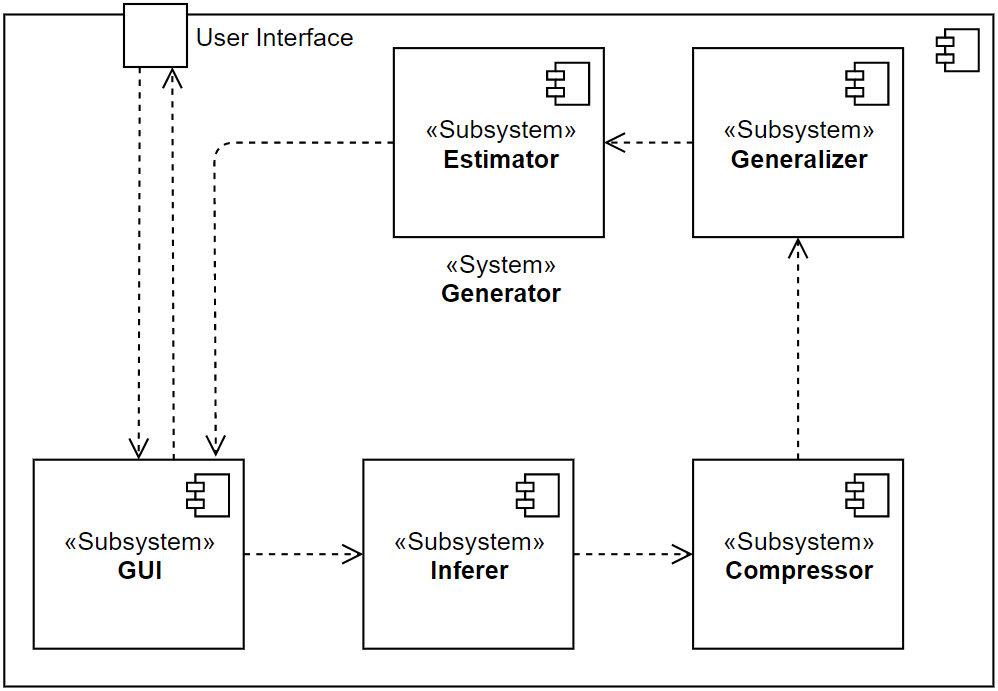
\includegraphics[width=12cm]{../images/Bausteinsicht_Ebene_1.PNG}
        \caption{Subsysteme mit fachlichen Abhängigkeiten}
    \end{figure}
    \underline{Ebene 2}
    \begin{figure}[H]
        \centering
        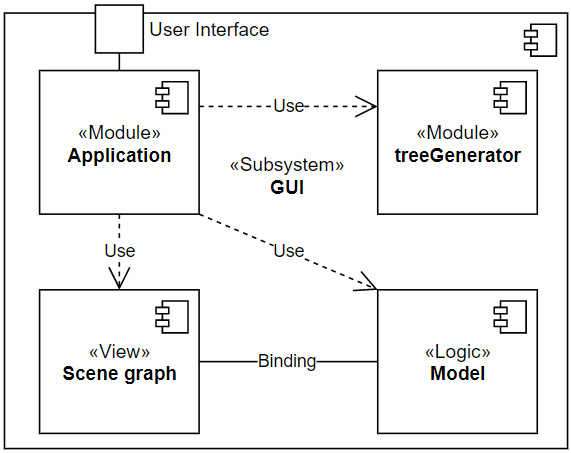
\includegraphics[width=9cm]{../images/Bausteinsicht_Ebene_2.PNG}
        \caption{Subsystem GUI}
    \end{figure}

    \subsection{Laufzeitsicht}
    \begin{figure}[H]
        \centering
        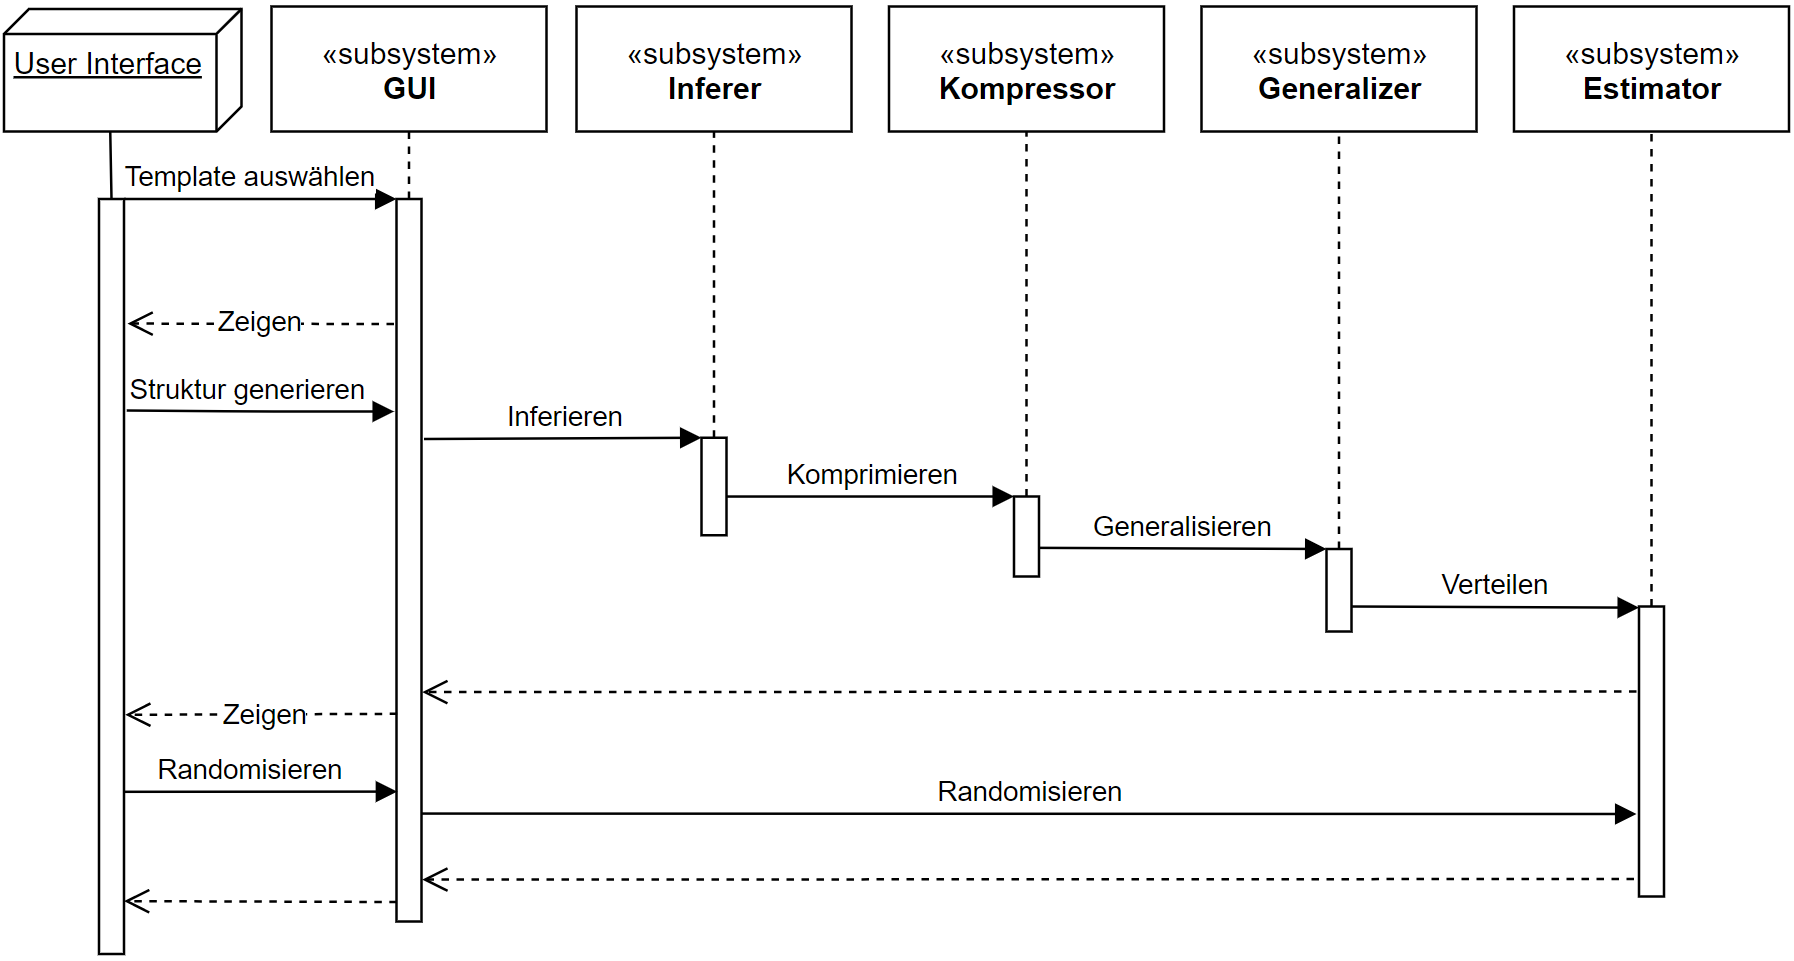
\includegraphics[width=14cm]{../images/Laufzeitsicht.PNG}
        \caption{Laufzeitsicht}
    \end{figure}

    \subsection{Verteilungsicht}
    \begin{figure}[H]
        \centering
        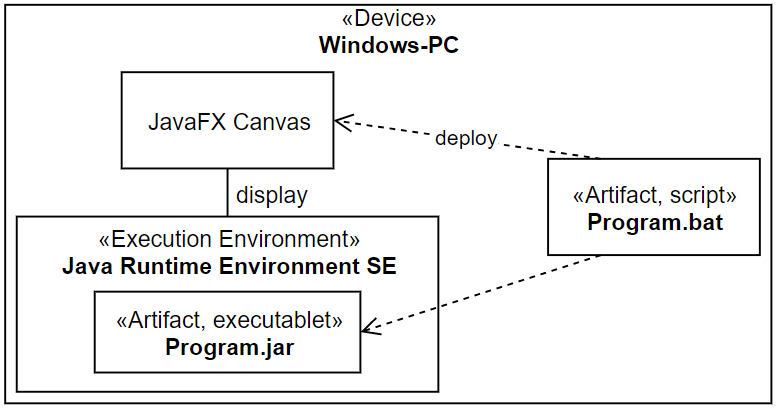
\includegraphics[width=10cm]{../images/Verteilungssicht.PNG}
        \caption{Infrastruktur Windows-PC}
    \end{figure}

    \subsection{Konzepte (todo)}
    \underline{Testbarkeit}\\~\\
    \underline{Validierung}\\~\\
    \underline{Fehlerbehandlung}
    \begin{itemize}
        \item Exception Handling
        \item Logging
    \end{itemize}
    \underline{Datenstrukturen}\\~\\
    \underline{Workflows}\\~\\
    \underline{Algorithmen}

    \subsection{Entscheidungen (todo)}
        \underline{Risiken}\\~\\
        \underline{Qualitätsmerkmale}\\~\\
        \underline{Alternativen}\\~\\
        \underline{Aufwand der Implementierung}

    \newpage

    \section{Releases}
    Dieses Kapitel beschreibt die Release-Planung des Softwareprojekts im Sinne eines XP-orientierten Ansatzes:\\
    Zuerst werden die Funktionalitäten, die im entsprechenden Release umgesetzt werden sollen definiert und \textbf{Epics}
    zugeteilt.
    Anschließend werden feingranulare User Stories formuliert, die mit einer Aufwandseinschätzung versehen werden.
    Mit diesen Informationen lässt sich dann die Iterationsplanung umsetzen.
    Die Umwandlung der User Stories in Arbeitsschritte (\textbf{Tasks}) und das Festlegen deren Dauer wird hier
    umgesetzt.\\~\\
    \underline{Beispiel: Release 1}\\~\\
    Erstellung einer grafischen Benutzeroberfläche zur Erstellung von Verzweigungsstrukturen\\
    \textit{Siehe Exposé Kapitel 1.1.2 Überblick Punkt I. Strukturieren und II. Visualisieren}
    
    \subsection{Planung}
    \begin{figure}[H]
        \centering
        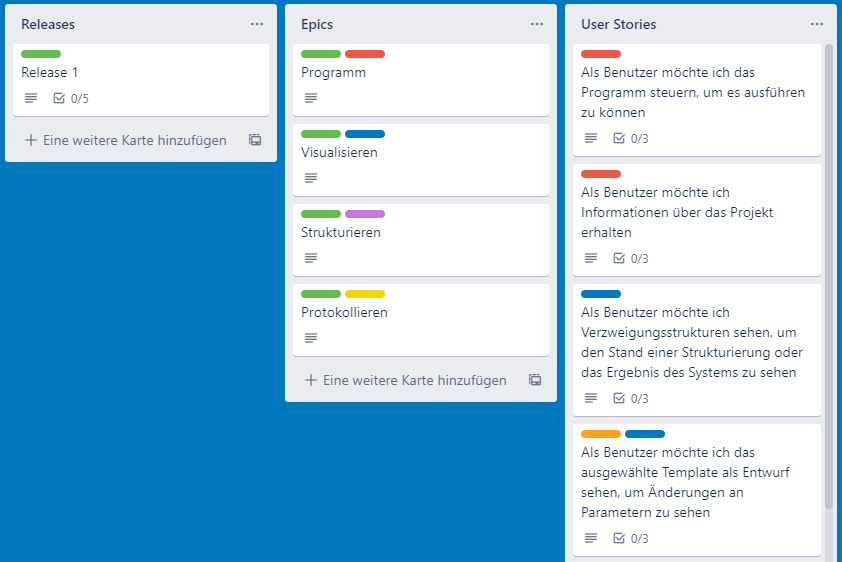
\includegraphics[width=12cm]{../images/User_Story_Map.PNG}
        \caption{Release-Planung: User Story Map mit Releases, Epics und User Stories}
    \end{figure}

    \newpage

    Release 1 enthält 4 Epics wird also in 4 Iterationen erarbeitet:
    \begin{itemize}
        \item Iteration 1 (Epic Programm, 2 User Stories), Gesamtdauer: 6h
    \end{itemize}
    \begin{figure}[H]
        \centering
        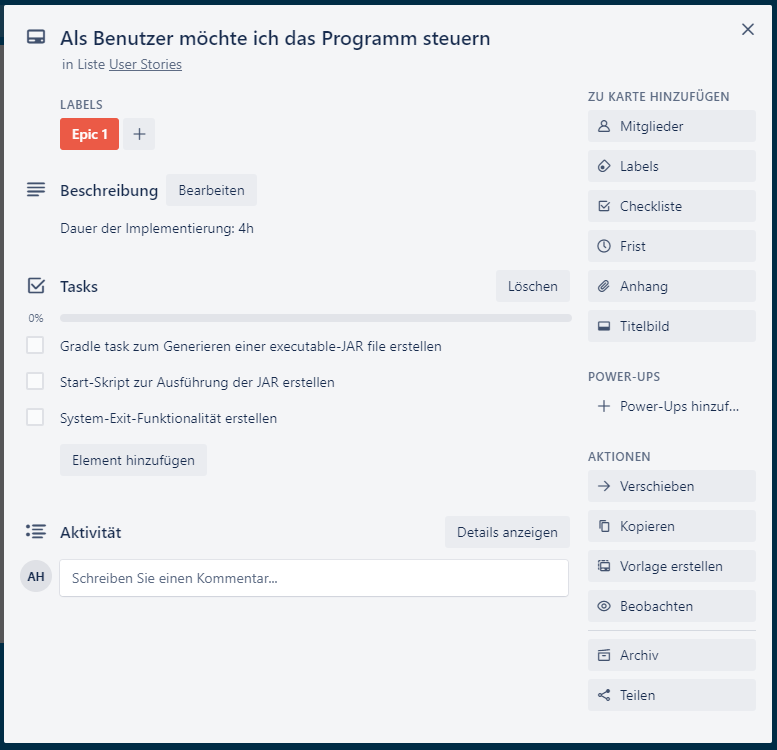
\includegraphics[width=12cm]{../images/User_Story_1.PNG}
        \caption{Iterationsplanung: User Story mit Tasks und Dauer}
    \end{figure}
    \begin{itemize}
        \item Iteration 2 (Epic Visualisieren, 2 User Stories), Dauer: 18h
        \item Iteration 3 (Epic Strukturieren, 5 User Stories), Dauer: 18h
        \item Iteration 4 (Epic Protokollieren, 1 User Story), Dauer: 2h
    \end{itemize}

    \newpage
    
    \subsection{Entwurf}
    Ein menschlicher Benutzer (\textbf{User}) nutzt das Programm, um eine Verzweigungsstruktur zu strukturieren.
    Hierzu wählt dieser einige Templates aus einer Sammlung vorgefertigter Templates aus, setzt Parameter und
    bestimmt den Ort der Platzierung.
    Die zu erstellende Struktur ist jeder Zeit sichtbar (Visualisierung).\\~\\
    Das System wird als Java-Programm mit main-Routine erstellt.\\~\\
    TODO

    \subsection{Testing}
    TODO

    \subsection{Programmierung}
    TODO

    \section{Implementation}
    Da die Arbeitspakete (Releases) iterativ und abgeschlossen erarbeitet werden, wird das
    \textbf{Pipeline} Design Pattern\cite{pipeline} genutzt.

    \newpage

    ~\nocite{*}
    \renewcommand{\refname}{Quellen}
    \bibliography{konzepte}
    \bibliographystyle{plain}
    \addcontentsline{toc}{section}{Quellen}

\end{document}